\section{Introduction}
\begin{itemize}
    \item Address classes A,B,C,D,E
    \item Important to understand for subnetting.
\end{itemize}


%----------------------------------------------------------------------------------------
\section{Class A IP Address}
\begin{itemize}
    \item Subnet Size:
        \begin{itemize}
            \item Class A, B, and C IPs are used to allocate addresses to our hosts.
            \item The bigger the host portion of the network, the more hosts we can have.
            \item If the subnet mask is /8, we have 24 bits available to allocate to hosts.
            \item If the subnet mask is /24, we only have 8 bits available to allocate to hosts.
        \end{itemize}
    
    \item How internet addressing was meant to work:
        \begin{itemize}
            \item The global coordination of internet IPv4 addressing is performed by IANA (Internet Assigned Numbers Authority).
                \begin{itemize}
                    \item Back when the designers were conceiving IPv4 they did not know that the internet was going to explode in popularity. There are some issues with IPv4 that would not make sense without context.
                \end{itemize}
            \item This is the way it was originally supposed to work:
            \item When a company wants to communicate on the internet, they apply for a range of IP addresses.
            \item If they have 6000 hosts, they ask for a range of IP addresses bug enough to convert that, plus room for growth.
            \item They then allocate their addresses to their hosts in their various offices.
            \item Unfortunately, when IPv4 was created, the designers didn't realise how big the internet was going to get, and they didn't create a big enough address space, this is why there is not enough addresses for everyone.
            \item The long term solution to this problem is IPv6 which has a much bigger address space.
            \item Private IP addresses with NAT (Network Address Translation) are currently deployed in the majority of enterprise networks as a workaround.
            \item You'll learn all about private addresses, NAT adn IPv6 in a later lecture.
            \item To understand the lectures until we get to that point, think about it from the context of the originally intended IPv4 design, where all hosts which can communicate on the internet have public IP addresses.
        \end{itemize}
    
    \item Class A:
        \begin{itemize}
            \item The internet authorities split the IPv4 address space into separate classes.
            \item Class A addresses are assigned to networks with a very large number of hosts.
                \begin{itemize}
                    \item In a class A there is going to be a small network portion and a large host portion.
                \end{itemize}
            \item The high-order (first) bit in class A address is always set to zero.
            \item The default subnet mask is /8.
            \item Valid networks addresses range from 1.0.0.0 to 126.0.0.0/8.
            \item This allows for 126 networks and 16,777,214 hosts per network.
                \begin{figure}[H]
                    \centering
                    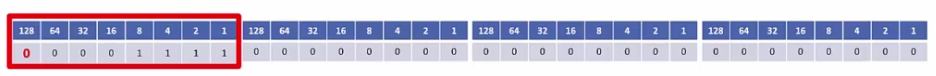
\includegraphics[width=0.4\textwidth]{./Figs/2022-01-08-20-28-34.png}
                % 	\caption{}
                \end{figure}
        \end{itemize}
    
    \item Reserved Class A Addresses:   
        \begin{itemize}
            \item The same exceptions apply for host allocation, all zeros and all ones are reserved.
            \item 0.0.0.0/8 is reserved and signifies 'this network'.
            \item 0.0.0.1 to 0.255.255.255 are not valid host addresses. Because the network portion is all 0s, as long as the network portion is 0 the rest cannot be used.
            \item 127.0.0.0/8 in the Class A space is reserved as the loopback address for testing the local computer.
            \item 127.0.0.0 to 127.255.255.255 are nto valid host addresses. 
                \begin{itemize}
                    \item 127.0.0.0 is used to test the IP stack on the local computer.
                \end{itemize}
            \item This means that because the first 8 bits cant be used when they are all set to 0 or when they are all set to 1, any combination of the host part is invalid if it begins in all 0s. This wiped out 33,554,428 addresses from the global address pool -- whops!
            \item They could have used just two address for this, but instead they chose the convention of all 0s and all 1s and ended up wiping out 16 million addresses twice. This is because the designers did not know that the internet was going to explode.
        \end{itemize}
    
    \item Using the loopback:
        \begin{itemize}
            \item Type ping 127.0.0.1 and you will ping the local IP stack:
                \begin{figure}[H]
                    \centering
                    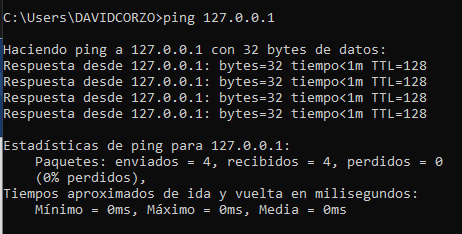
\includegraphics[width=0.4\textwidth]{./Figs/2022-01-08-20-43-19.png}
                % 	\caption{}
                \end{figure}
            
            \item But since the entire network address starting in 127 is reserved any combination of digits after the 127 are going to be ignored and you would be pining the local IP stack, this is why we lost 16 million IP addresses. So here I can invent any number, as long as it starts with 127.X.X.X it will reference the same reserved loopback address.
                \begin{figure}[H]
                    \centering
                    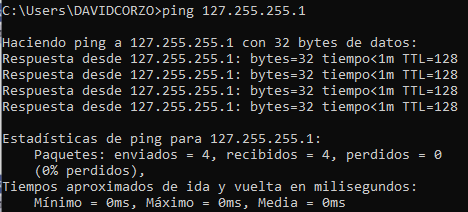
\includegraphics[width=0.4\textwidth]{./Figs/2022-01-08-20-45-04.png}
                % 	\caption{}
                \end{figure}
        \end{itemize}
    
    \item Subnetting:
        \begin{itemize}
            \item Obviously a company wouldn't put all 16,777,214 hosts into a single logical network, this would be terrible for performance and security.
            \item They would split their /8 address allocation into smaller subnets and allocate these to different offices adn types of hosts.
            \item For example if they recieved 15.0.0.0/8, they could allocate the subnet 15.0.1.0/24 to sales computers in New York, 15.0.2.0/24 to accounting PC's and 15.0.9.0/24 to sales computers in Boston. 
            \item This is called subnetting and you'll master it later in this section.
            \item So they would have that huge network that they got assigned by the internet authorities and they can now assign it to their different offices and hosts. This is called subnetting.
        \end{itemize}
\end{itemize}


%----------------------------------------------------------------------------------------
\section{IP addresses class B and C}
\begin{itemize}
    \item Class B:
        \begin{itemize}
            \item Class B addresses are assigned to medioum-sized to large sized networks.
            \item The two high-order bits in a class B address are always set to binary 1 0. 
            \item The default subnet mask is /16.
            \item Valid network addresses range from 128.0.0.0 to 191.255.0.0/16.
            \item This allows fro 16,384 networks and 65,534 hosts per network.
            \item This would also be subnetted in a real world environment.
                \begin{figure}[H]
                    \centering
                    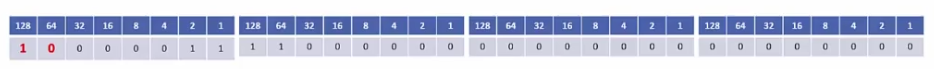
\includegraphics[width=0.4\textwidth]{./Figs/2022-01-08-20-52-48.png}
                % 	\caption{}
                \end{figure}
            \item 131.192.0.0/16.
        \end{itemize}
\end{itemize}
